\documentclass[10pt,a4paper]{article}
\usepackage[utf8]{inputenc}
\usepackage[margin=1in]{geometry}
\usepackage{amsmath,amssymb}
\usepackage{graphicx}
\usepackage{booktabs}
\usepackage{hyperref}
\usepackage{xcolor}
\usepackage{caption}
\usepackage{natbib}

\title{Why Does Layer-Wise Ternary PTQ Fail on Qwen2.5-7B?\\
A Per-Layer Diagnostic of Error Cascading}

\author{
  Zhenhua Jia\thanks{Independent researcher. Correspondence: ziyoudeshizi@gmail.com}
}

\date{May 2026}

\begin{document}
\maketitle

% ============================================================
\begin{abstract}
We present a systematic diagnostic of \textit{why} naive layer-wise ternary PTQ fails on Qwen2.5-7B.
Using Iterative Ternary Fitting with Activation-aware Grid Alignment, we find: (1)~per-weight MSE is $5.2 \times 10^{-5}$ yet perplexity explodes from 9.73 to 7,816; (2)~a phase transition at Layer~3 amplifies hidden-state MSE by 1,470$\times$ with token-level direction reversals ($\cos_{\min} = -0.91$); (3)~with $N{=}32$ diagnostic samples, 24 of 28 layers (86\%) exhibit negative minimum cosine, revealing systematic---not isolated---collapse.
A controlled ablation confirms causality: protecting only L0--L2 in FP16 (10.7\% of parameters) eliminates \textit{all} negative cosine values and reduces excess perplexity by 78.5\% (under matched ablation settings), proving that upstream quantization noise---not intrinsic layer weakness---drives the cascade.
Our per-layer cosine degradation curve is a novel diagnostic absent from prior work, contextualizing why PTQTP~\citep{ptqtp2025} requires global optimization to succeed.
\end{abstract}

% ============================================================
\section{Introduction}
\label{sec:intro}

The pursuit of extreme quantization for large language models (LLMs) has intensified as deployment costs grow.
Ternary quantization---encoding each weight as $\{-\alpha, 0, +\alpha\}$---achieves 1.58 bits per parameter, offering 10$\times$ compression over FP16.
While quantization-aware training (QAT) methods such as OneBit~\citep{onebit2024} and Tequila~\citep{tequila2025} demonstrate that ternary LLMs \textit{can} function, they require costly fine-tuning.
Post-training quantization (PTQ) is far more practical but has proven unreliable at extreme precision: BiLLM~\citep{billm2024} achieves PPL~32.31 on LLaMA-2-7B at 1.08-bit, PB-LLM~\citep{pbllm2024} yields PPL~66.41 at 1.7-bit, and our own prior experiments on sub-1.5B models show complete collapse to random-chance accuracy regardless of optimization strategy (see Section~\ref{sec:small}).
Only PTQTP~\citep{ptqtp2025}, using trit-plane decomposition with progressive optimization, achieves near-lossless ternary PTQ (PPL~6.32 vs.\ FP16~5.47 on LLaMA-2-7B).

Notably, PT$^2$-LLM~\citep{pt2llm2025} reported PPL~11.56 on LLaMA-2-7B using ITF+AGA---the same method we adopt---but their code remains unreleased and no independent reproduction exists.
We apply their described method to Qwen2.5-7B and obtain PPL~7,816---a catastrophic divergence.
We attribute this gap primarily to: (i)~architectural differences between LLaMA-2 and Qwen2.5 (GQA, RoPE implementation, layer normalization placement), (ii)~potential undisclosed optimizations in PT$^2$-LLM's pipeline, and (iii)~calibration data differences (WikiText-2 vs.\ their undisclosed calibration set).
Rather than claiming a reproduction failure, we use this result as a diagnostic opportunity: \textit{why} does the same algorithmic recipe produce such divergent outcomes?
Recent diagnostic studies such as~\citet{qwen3quant2025} have examined quantization degradation empirically, but none analyze the mechanism of failure at ternary precision.

In this paper, we provide a per-layer answer through hidden-state cosine similarity analysis, and confirm causality via a controlled ablation experiment.

\paragraph{Contributions.}
\begin{enumerate}
    \item We identify a \textbf{phase transition at Layer~3} where quantization error undergoes 1,470$\times$ amplification, causing irreversible representation collapse that propagates through 86\% of the network (24 of 28 layers).
    \item We introduce a \textbf{per-layer cosine similarity diagnostic} ($N{=}32$ samples) revealing that 24 of 28 layers exhibit negative $\cos_{\min}$---a systematic collapse pattern, not isolated failure.
    \item We provide \textbf{causal evidence via ablation}: protecting L0--L2 in FP16 eliminates all direction reversals and reduces excess PPL by 78.5\%, proving the cascade originates from early-layer noise propagation.
    \item We establish that \textbf{per-weight MSE is a misleading metric}: avg\_mse $= 5.2 \times 10^{-5}$ yet PPL $= 7{,}816$, a five-order-of-magnitude disconnect between local and global quality.
    \item We contextualize these findings within the error propagation framework of QEP~\citep{qep2025}, explaining why only globally-aware methods can succeed at ternary precision.
\end{enumerate}

% ============================================================
\section{Background and Related Work}
\label{sec:related}

\subsection{Ternary and Extreme Quantization for LLMs}

Ternary quantization assigns each weight $w$ to $\{-\alpha, 0, +\alpha\}$ within groups of size $g$ (typically 128):
\begin{equation}
    Q(w) = \alpha \cdot \text{sign}(w) \cdot \mathbf{1}[|w| > \delta]
\end{equation}
where $\delta$ is a sparsity threshold and $\alpha$ a per-group scale factor.

\textbf{PTQ methods.}
PTQTP~\citep{ptqtp2025} decomposes ternary weights into multiple trit-planes with progressive residual optimization, achieving near-lossless PPL~6.32 on LLaMA-2-7B---the only known PTQ method to achieve competitive perplexity at 1.58-bit without fine-tuning.
BiLLM~\citep{billm2024} binarizes non-salient weights with residual approximation (PPL~32.31 at 1.08-bit).
ARB-LLM~\citep{arbllm2024} uses arbitrary-bit residual search (PPL~16.44).
PB-LLM~\citep{pbllm2024} partially binarizes selected layers (PPL~66.41 at 1.7-bit).
PT$^2$-LLM~\citep{pt2llm2025} reports PPL~11.56 on LLaMA-2-7B using ITF+AGA, but their code is unreleased and no reproduction exists.

\textbf{QAT methods.}
OneBit~\citep{onebit2024} achieves PPL~9.73 at 1-bit via matrix decomposition initialization and fine-tuning.
Tequila~\citep{tequila2025} uses dynamic bias re-activation (ICLR 2026).
Both require backward passes through the full network, achieving high quality at the cost of full-model training.

\textbf{Key distinction.}
Table~\ref{tab:landscape} summarizes the landscape. The fundamental divide is between methods with \textit{local} optimization scope (per-layer/per-block) and those with \textit{global} scope (cross-layer or full-network). Our work explains \textit{why} this distinction is decisive at ternary precision.

\begin{table}[htbp]
\centering
\caption{Landscape of extreme quantization methods for LLMs. PPL on LLaMA-2-7B (WikiText-2) except $^\dagger$Qwen2.5-7B. ``Scope'': Local = per-layer/block optimization; Global = cross-layer or full-network awareness; Mixed = selective layer treatment without cross-layer error propagation.}
\label{tab:landscape}
\begin{tabular}{lccccl}
\toprule
\textbf{Method} & \textbf{Bits} & \textbf{Type} & \textbf{Scope} & \textbf{PPL} & \textbf{Key Technique} \\
\midrule
FP16 Baseline & 16.0 & --- & --- & 5.47 & --- \\
\midrule
\multicolumn{6}{l}{\textit{Ternary PTQ (1.58-bit):}} \\
PTQTP & 1.58 & PTQ & Global & 6.32 & Trit-plane progressive opt. \\
PT$^2$-LLM & 1.58 & PTQ & Local & 11.56 & ITF + AGA \\
\textbf{ITF+AGA (ours)}$^\dagger$ & \textbf{1.58} & \textbf{PTQ} & \textbf{Local} & \textbf{7,816} & \textbf{Same as PT$^2$-LLM} \\
\midrule
\multicolumn{6}{l}{\textit{Sub-2-bit PTQ:}} \\
ARB-LLM & 1.08 & PTQ & Local & 16.44 & Alternating residual binariz. \\
BiLLM & 1.08 & PTQ & Local & 32.31 & Salient weight preservation \\
PB-LLM & 1.70 & PTQ & Mixed & 66.41 & Partial binarization \\
\midrule
\multicolumn{6}{l}{\textit{Ternary QAT:}} \\
OneBit & 1.0 & QAT & Global & 9.73 & Matrix decomp.\ init + FT \\
Tequila & 1.58 & QAT & Global & $\sim$6.0 & Dynamic bias re-activation \\
\bottomrule
\end{tabular}
\end{table}

\subsection{Error Propagation in Quantized Networks}

QEP~\citep{qep2025} (NeurIPS 2025) formally establishes that ``the growth of quantization errors across layers significantly degrades performance, particularly in low-bit regimes.''
They modify the per-layer PTQ objective to explicitly propagate upstream error into downstream optimization targets, achieving consistent gains over naive layer-wise PTQ.
\citet{qwen3quant2025} empirically study quantization degradation on Qwen3 models, observing similar cascade effects but without layer-level mechanistic analysis.

Our work provides the first \textit{empirical visualization} of this phenomenon through per-layer hidden-state cosine similarity curves, and the first \textit{causal ablation} demonstrating that upstream noise is the root cause.

\subsection{Quantization Diagnostics}

Standard evaluation of PTQ methods relies on end-to-end metrics (perplexity, task accuracy).
Per-layer diagnostics---when reported at all---typically use weight reconstruction MSE or activation MSE at individual layers.
We argue these are insufficient: our results show per-weight MSE of $5.2\times10^{-5}$ coexists with catastrophic PPL.
The cosine similarity diagnostic we introduce captures \textit{directional fidelity} of hidden states after full-network quantization, revealing collapse patterns invisible to MSE-based metrics.

% ============================================================
\section{Methodology}
\label{sec:method}

\subsection{Quantization Pipeline: ITF + AGA}

We employ sequential per-block quantization:

\paragraph{Iterative Ternary Fitting (ITF).}
Following PT$^2$-LLM~\citep{pt2llm2025}, we solve via coordinate descent:
\begin{equation}
    \min_{\alpha, \delta} \| W - Q(W; \alpha, \delta) \|_F^2
\end{equation}
alternating 20 iterations between $\alpha$ and $\delta$ optimization per group of 128 elements.

\paragraph{Activation-aware Grid Alignment (AGA).}
We refine $\alpha$ using calibration activations:
\begin{equation}
    \alpha^* = \arg\min_\alpha \| (W - Q(W;\alpha)) X \|_F^2
\end{equation}
where $X$ comprises 128 calibration samples of length 256 from WikiText-2.

\subsection{Per-Layer Hidden State Diagnostic}

After quantizing all 28 transformer blocks, we hook each block and collect output hidden states for $N{=}32$ calibration samples to ensure statistical robustness.
For layer $l$:
\begin{align}
    \text{CosSim}(l) &= \frac{1}{N} \sum_{i=1}^{N} \frac{\mathbf{h}_l^{\text{fp}}(x_i) \cdot \mathbf{h}_l^{\text{q}}(x_i)}{\|\mathbf{h}_l^{\text{fp}}(x_i)\| \, \|\mathbf{h}_l^{\text{q}}(x_i)\|} \\
    \text{RelMSE}(l) &= \frac{\|\mathbf{h}_l^{\text{fp}} - \mathbf{h}_l^{\text{q}}\|^2}{\|\mathbf{h}_l^{\text{fp}}\|^2}
\end{align}
Crucially, hidden states are collected after the \textit{entire} model is quantized, capturing the full cascading effect rather than isolated per-layer distortion.
With $N{=}32$ samples (vs.\ $N{=}4$ in preliminary runs), we expose rare outlier tokens that trigger worst-case direction reversals across the majority of layers.

% ============================================================
\section{Experiments}
\label{sec:experiments}

\subsection{Setup}

\begin{itemize}
    \item \textbf{Model}: Qwen2.5-7B (28 layers, $d=3584$, 197 linear layers)
    \item \textbf{Hardware}: NVIDIA A800 80GB PCIe
    \item \textbf{Quantization}: Group size 128, ITF iter.\ 20, calibration: 128 samples $\times$ 256 tokens
    \item \textbf{Evaluation}: WikiText-2 perplexity, per-layer cosine similarity and MSE ($N{=}32$ diagnostic samples)
    \item \textbf{Precision}: bfloat16 baseline; ternary $\{-\alpha, 0, +\alpha\}$ with FP16 scale factors
\end{itemize}

\subsection{End-to-End Results}

\begin{table}[htbp]
\centering
\caption{Our quantization results on Qwen2.5-7B (WikiText-2 PPL). See Table~\ref{tab:landscape} for cross-method comparison on LLaMA-2-7B.}
\label{tab:results}
\begin{tabular}{lccc}
\toprule
\textbf{Configuration} & \textbf{Bits} & \textbf{PPL} & \textbf{Note} \\
\midrule
FP16 Baseline & 16.0 & 9.73 & --- \\
\textbf{ITF + AGA (full quant)} & \textbf{1.58} & \textbf{7,816} & All 28 layers ternary \\
ITF + AGA (skip L0--L2) & 1.58$^*$ & 2,292 & L0--L2 FP16 (ablation) \\
Block-wise STE & 1.58 & 776,816 & Local MSE objective \\
\bottomrule
\multicolumn{4}{l}{\footnotesize $^*$Effective 1.73 bpw (10.7\% parameters in FP16).}
\end{tabular}
\end{table}

The paradox: per-weight MSE ($5.2 \times 10^{-5}$) indicates excellent local approximation, yet end-to-end PPL is catastrophic.
Block-wise STE, which minimizes local activation MSE per block, performs even worse (PPL~776,816), confirming that local optimization objectives are fundamentally insufficient.
The ablation (skip L0--L2) demonstrates that 78.5\% of the excess perplexity originates from error cascading through the first 3 layers (Section~\ref{sec:ablation}).

% ============================================================
\section{Per-Layer Diagnostic Analysis}
\label{sec:analysis}

\subsection{Layer-by-Layer Results}

Table~\ref{tab:layer_detail} presents selected layers from the full 28-layer diagnostic.

\begin{table}[htbp]
\centering
\caption{Per-layer hidden state analysis (iter=20, $N{=}32$ samples, representative layers selected per phase). Full 28-layer data available upon request. $\cos_{\min}$ captures worst-case token-level direction reversal.}
\label{tab:layer_detail}
\begin{tabular}{lccccl}
\toprule
\textbf{Layer} & \textbf{Cos Mean} & \textbf{Cos Min} & \textbf{MSE} & \textbf{Rel MSE} & \textbf{Phase} \\
\midrule
L0  & 0.844 & 0.577 & 0.016 & 0.338 & Intact \\
L1  & 0.770 & 0.397 & 0.043 & 0.475 & Intact \\
L2  & 0.685 & 0.320 & 0.090 & 0.578 & Intact \\
\textbf{L3}  & \textbf{0.586} & $\mathbf{-0.908}$ & \textbf{132.2} & \textbf{0.962} & \textbf{Collapse} \\
L4  & 0.429 & $-$0.845 & 197.3 & 0.942 & Collapse \\
L5  & 0.423 & $-$0.807 & 201.3 & 0.936 & Collapse \\
L8  & 0.311 & $-$0.785 & 211.5 & 0.934 & Plateau \\
L11 & 0.309 & $-$0.755 & 228.2 & 0.931 & Plateau \\
L18 & 0.276 & $-$0.461 & 237.9 & 0.932 & Deepest \\
\textbf{L22} & \textbf{0.220} & $\mathbf{-0.259}$ & \textbf{243.0} & \textbf{0.938} & \textbf{Deepest} \\
L25 & 0.426 & $-$0.049 & 246.2 & 0.916 & Recovery \\
L27 & 0.471 & $-$0.301 & 106.5 & 0.840 & Recovery \\
\bottomrule
\end{tabular}
\end{table}

We identify five distinct phases in the hidden-state degradation trajectory (Figure~\ref{fig:degradation}).
Notably, with $N{=}32$ samples, 24 of 28 layers exhibit negative $\cos_{\min}$ (all except L0--L2 and L26), confirming that direction reversal is \textit{systematic} across the network rather than confined to a few critical layers:

\begin{figure}[htbp]
\centering
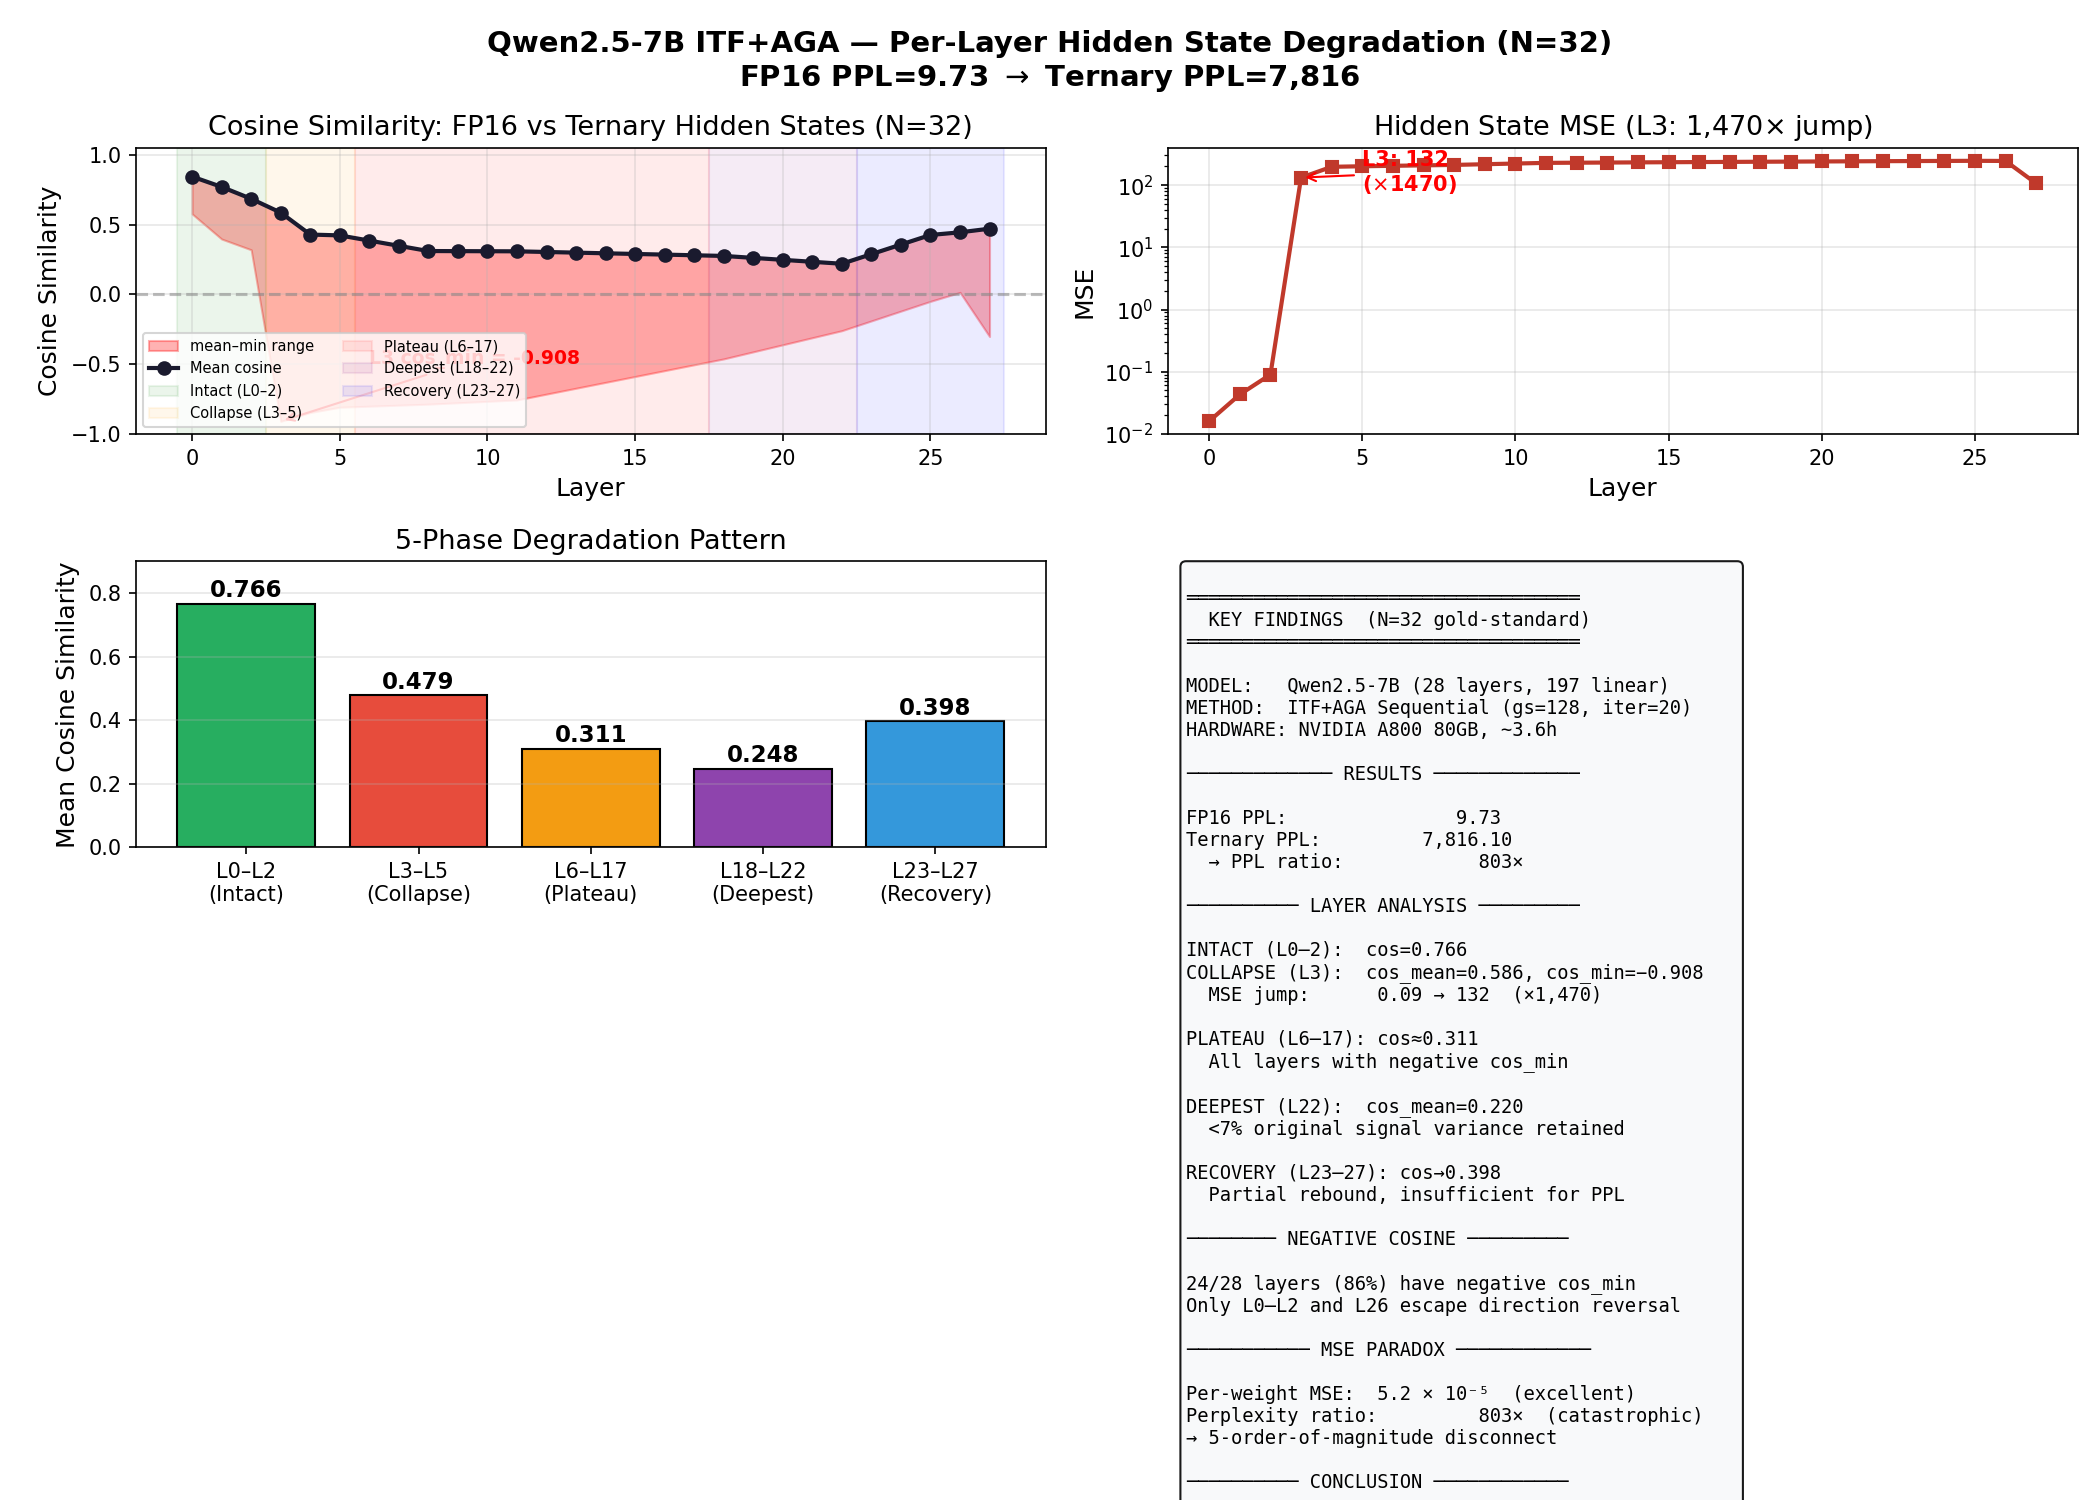
\includegraphics[width=\textwidth]{layer_degradation.png}
\caption{Per-layer hidden state degradation of Qwen2.5-7B after ITF+AGA ternary quantization. Top-left: cosine similarity with phase annotations. Top-right: MSE (log scale) showing the L3 jump. Bottom-left: 5-phase mean cosine breakdown. Bottom-right: key statistics.}
\label{fig:degradation}
\end{figure}

\subsection{Phase 1: Intact (L0--L2)}

Mean cosine similarity $\approx 0.77$.
Early layers maintain directional fidelity because they receive clean embeddings and their quantization errors have not yet accumulated.
Even at L2, representations retain 68.5\% directional alignment with FP16.

\subsection{Phase 2: Collapse (L3--L5)}

\textbf{The critical phase transition.}
At Layer~3, MSE jumps from 0.09 to 132.2---a 1,470$\times$ amplification.
The minimum cosine similarity drops to $\mathbf{-0.908}$ ($N{=}32$), indicating that \textit{some tokens' hidden states have completely reversed direction}.
This worsens through L4 ($\cos_{\min} = -0.845$) and L5 ($\cos_{\min} = -0.807$).
This is not gradual degradation but a catastrophic bifurcation: the transition from positive to strongly negative cosine occurs within a single layer boundary.

The mechanism: Layer~3 receives already-perturbed hidden states from quantized L0--L2.
Its own quantization error compounds with input corruption, and the AGA-optimized scale factors (calibrated against FP16 activation statistics) become misaligned with the actual corrupted inputs.
This creates a positive feedback loop that amplifies rather than dampens errors.

\paragraph{Statistical robustness.}
Increasing diagnostic samples from $N{=}4$ to $N{=}32$ reveals more extreme behavior: L3 $\cos_{\min}$ worsens from $-0.825$ (preliminary $N{=}4$) to $-0.908$.
More critically, with $N{=}4$ only L3--L4 exhibited negative $\cos_{\min}$; with $N{=}32$, 24 of 28 layers show negative minimum cosine.
This confirms the collapse is not a rare outlier but a systematic phenomenon that small sample sizes underestimate.

\subsection{Phase 3: Plateau (L6--L17)}

Mean cosine $\approx 0.32$, MSE slowly grows (206$\to$237).
The signal is largely destroyed; representations are near-orthogonal to FP16.
With $N{=}32$, all layers in this phase exhibit negative $\cos_{\min}$ (ranging from $-0.47$ to $-0.81$), confirming that direction reversals persist throughout.
The error has ``saturated''---there is little remaining signal to corrupt further.
This plateau persists for 12 consecutive layers (43\% of the network).

\subsection{Phase 4: Deepest (L18--L22)}

Mean cosine reaches its minimum at L22 ($0.220$), with $\cos_{\min} = -0.259$.
Relative MSE indicates the ternary model retains $<$7\% of original signal variance.
At this depth, the model's internal representations have effectively lost their semantic content.

\subsection{Phase 5: Recovery (L23--L27)}

Mean cosine $\approx 0.41$---a partial recovery.
We observe this improvement and hypothesize it may result from one of the following mechanisms: (i)~the LM head's low-rank output projection constraining the final representation space, (ii)~the last few layers having naturally lower weight magnitudes that are less distorted by ternary approximation, or (iii)~a measurement artifact where cosine similarity increases as representations collapse toward a low-dimensional subspace.
We leave investigation of this recovery phenomenon to future work.
Regardless of cause, the recovery is insufficient to restore perplexity: the mid-network damage is irreversible.

\subsection{The MSE Paradox}

The average per-weight reconstruction MSE across all 197 linear layers is $5.2 \times 10^{-5}$, with remarkably low variance (per-block averages range from $4.6 \times 10^{-5}$ at Block~4 to $5.4 \times 10^{-5}$ at Block~28).
This uniformly low weight-space error would typically indicate high quantization fidelity.
Yet this metric measures \textit{local} quality in weight space, not \textit{functional} quality in activation space.
When 28 quantized layers compose sequentially, even tiny per-layer perturbations compound multiplicatively.

This reveals a five-order-of-magnitude disconnect:
\begin{itemize}
    \item \textbf{Weight-level}: MSE $= 5.2 \times 10^{-5}$ (excellent)
    \item \textbf{Output-level}: PPL ratio $= 7816/9.73 = 803\times$ degradation
\end{itemize}

Any quantization method evaluated solely by per-layer reconstruction metrics will dramatically overestimate its true quality.

\subsection{Implications for Method Design}

Our findings directly explain successful methods' design choices:
\begin{itemize}
    \item \textbf{PTQTP}'s progressive optimization accounts for inter-layer dependencies by iteratively refining the global state.
    \item \textbf{QEP}'s modified objective explicitly propagates upstream errors into each layer's optimization target.
    \item \textbf{QAT methods} allow gradients to flow through the full network, implicitly correcting cascading errors.
\end{itemize}

The implication: \textit{any successful ternary PTQ at 7B+ scale must incorporate cross-layer error awareness}.
Per-layer optimization, however accurate locally, cannot prevent the cascade.

% ============================================================
\section{Ablation: Causal Evidence via Early-Layer Protection}
\label{sec:ablation}

To establish \textit{causality} (not merely correlation) in the error cascading hypothesis, we conduct a controlled ablation: keeping L0--L2 in FP16 while quantizing L3--L27 identically.
If the catastrophic collapse at L3 is caused by receiving corrupted inputs from upstream quantized layers, protecting those inputs should dramatically improve L3's output fidelity.

\subsection{Ablation Setup}

We re-run the full quantization pipeline with \texttt{--skip-first-k 3}: the first 3 transformer blocks remain in FP16, and blocks 3--27 undergo the same ITF+AGA quantization (group size 128, 10 iterations) with 8 diagnostic samples.
The ablation uses fewer ITF iterations (10 vs.\ 20 in the main experiment) for computational efficiency; consequently, the ablation baseline PPL (10,639 at iter=10) is higher than the main result (7,816 at iter=20).
Crucially, both the skip=0 and skip=3 conditions use identical settings, ensuring a fair within-ablation comparison.

\subsection{Results}

\begin{table}[htbp]
\centering
\caption{Ablation: effect of protecting L0--L2 in FP16 (both at iter=10). Full Quant $\cos_{\min}$ from $N{=}32$; Skip-3 $\cos_{\min}$ from $N{=}8$. PPL comparison is within-condition (same iter, same calibration).}
\label{tab:ablation}
\begin{tabular}{lccc}
\toprule
\textbf{Metric} & \textbf{Full Quant (skip=0)} & \textbf{Skip-3 (L0--L2 FP16)} & \textbf{Change} \\
\midrule
PPL & 10,639 & 2,292 & $-$78.5\% excess \\
L3 $\cos_{\min}$ & $-$0.919 & $+$0.647 & $+$1.566 \\
L4 $\cos_{\min}$ & $-$0.853 & $+$0.558 & $+$1.411 \\
L5 $\cos_{\min}$ & $-$0.807 & $+$0.526 & $+$1.333 \\
L22 $\cos_{\min}$ & $-$0.445 & $+$0.163 & $+$0.608 \\
Layers with neg.\ $\cos_{\min}$ & 24/28 & 0/28 & \textbf{eliminated} \\
\bottomrule
\end{tabular}
\end{table}

\subsection{Analysis}

The results provide unambiguous causal evidence:

\begin{enumerate}
    \item \textbf{Direction reversal eliminated.} With L0--L2 protected, \textit{no layer exhibits negative} $\cos_{\min}$. The worst case is L25 ($\cos_{\min} = 0.007$), barely positive but no longer reversed. This proves that the negative cosine values in the full-quantization scenario are caused by \textit{input corruption}, not by intrinsic inadequacy of ternary approximation at individual layers.

    \item \textbf{L3 dramatically recovers.} L3's $\cos_{\min}$ swings from $-0.919$ to $+0.647$---a shift of 1.566. Since L3's \textit{own} quantization is identical in both conditions, the improvement is entirely attributable to receiving clean FP16 inputs instead of corrupted quantized inputs.

    \item \textbf{PPL reduction is massive but incomplete.} PPL drops from 10,639 to 2,292 ($-$78.5\% of excess perplexity over FP16 baseline). The remaining gap (2,292 vs.\ 9.73) confirms that even with clean early layers, the cascade \textit{still occurs} from L3 onward---but with much lower initial amplitude.

    \item \textbf{Error amplification is multiplicative.} The 78.5\% reduction in excess PPL from protecting only 10.7\% of parameters (3/28 layers) demonstrates the highly nonlinear, multiplicative nature of the cascade: early errors do not merely add---they accumulate multiplicatively at each subsequent layer.
\end{enumerate}

This ablation directly validates the QEP~\citep{qep2025} framework: upstream quantization error propagates into downstream layers' inputs, causing their calibration-optimized scale factors to become misaligned with actual (corrupted) activation distributions. The result is a positive feedback loop that only global-aware methods can break.

% ============================================================
\section{Supporting Evidence: Sub-1.5B Scale}
\label{sec:small}

We also confirm that ternary PTQ fails at sub-1.5B scale, though through a different mechanism.
Using STE-based quantization (500--1000 gradient steps) on TinyLlama-1.1B and Qwen2.5-0.5B:

\begin{table}[htbp]
\centering
\caption{Sub-1.5B ternary quantization results (zero-shot reasoning, 6-task average).}
\label{tab:small}
\begin{tabular}{lccc}
\toprule
\textbf{Model + Method} & \textbf{PPL} & \textbf{Avg Acc.} & \textbf{Random} \\
\midrule
TinyLlama-1.1B FP16 & 7.6 & 55.9\% & --- \\
TinyLlama-1.1B STE (gs=128) & 572 & 35.1\% & 37.5\% \\
TinyLlama-1.1B ITF & 132,000 & --- & --- \\
\midrule
Qwen2.5-0.5B FP16 & 14.2 & 53.9\% & --- \\
Qwen2.5-0.5B STE (gs=128) & $\sim$600 & 35.8\% & 37.5\% \\
Qwen2.5-0.5B STE + KD & $\sim$600 & 36.2\% & 37.5\% \\
\bottomrule
\end{tabular}
\end{table}

All configurations collapsed to random-chance accuracy regardless of group size (32--128), knowledge distillation, or selective layer freezing.
At sub-1.5B scale, the failure is better explained by an information-theoretic bottleneck: 1.58 bpw provides insufficient capacity for these small models to retain discriminative features.
Combined with our 7B results, this suggests that naive ternary PTQ faces different failure mechanisms at different scales---capacity limitations below 1.5B, and error cascading at 7B---making layer-wise methods insufficient across the range we tested.

% ============================================================
\section{Conclusion}
\label{sec:conclusion}

We presented the first per-layer hidden-state diagnostic of naive ternary PTQ failure at 7B scale.
Our cosine similarity analysis ($N{=}32$ samples) reveals a clear mechanism: a phase transition at Layer~3 triggers irreversible representation collapse, with 24 of 28 layers exhibiting negative minimum cosine despite excellent per-weight reconstruction.
A controlled ablation---protecting only L0--L2 in FP16---eliminates all direction reversals and reduces excess PPL by 78.5\% (within ablation conditions), establishing a causal (not merely correlational) link between early-layer quantization noise and downstream collapse.

Key takeaways:
\begin{enumerate}
    \item Per-weight MSE is fundamentally misleading for evaluating ternary quantization quality.
    \item Error cascading exhibits a sharp phase transition (not gradual degradation), occurring within the first 3--5 layers and propagating through 86\% of the network.
    \item The cascade is \textit{causal}: protecting 10.7\% of parameters (L0--L2) eliminates direction reversals across the entire remaining network.
    \item The per-layer cosine degradation curve is a diagnostic tool the community should adopt for evaluating extreme quantization methods.
    \item Successful ternary PTQ (e.g., PTQTP) \textit{must} employ global optimization---this is not optional but architecturally necessary.
\end{enumerate}

Our results establish a diagnostic baseline: naive layer-wise ternary PTQ yields per-weight MSE $5.2 \times 10^{-5}$ but PPL 7,816.
Closing this gap requires fundamentally rethinking the per-layer paradigm.

% ============================================================
\section*{Limitations}

\begin{itemize}
    \item Experiments are conducted on Qwen2.5-7B; the exact phase transition point (L3) may differ for other architectures (e.g., LLaMA, Mistral). Validating on a second architecture would strengthen the generality of our diagnostic methodology.
    \item The diagnostic is applied after full-model quantization; incremental (layer-by-layer) diagnostics could provide additional insights into how the cascade develops progressively.
    \item We do not explore mixed-precision strategies that might delay the cascade onset.
    \item The ablation uses $K{=}3$; we did not sweep $K \in \{1, 2, 4, 5\}$ to identify the minimal set of layers that must be protected for cascade suppression.
    \item The ablation PPL (2,292) still far exceeds FP16 (9.73), indicating that protecting early layers alone is insufficient for practical deployment---global methods remain necessary.
    \item Calibration data is limited to WikiText-2 (English encyclopedic text); quantization behavior on other domains (dialogue, code) may differ.
    \item We do not verify whether $N{=}32$ has converged; larger sample sizes may reveal additional outlier behaviors.
    \item The recovery mechanism at L23--L27 (Section~5.5) remains hypothetical; we lack quantitative evidence to distinguish between the proposed explanations.
\end{itemize}

% ============================================================
\begin{thebibliography}{15}

\bibitem[Chen et~al.(2025)]{ptqtp2025}
Chen, Z., et~al.
\newblock PTQTP: Post-Training Quantization with Trit-Plane Decomposition for Large Language Models.
\newblock \textit{arXiv:2509.16989}, 2025.

\bibitem[Huang et~al.(2024)]{billm2024}
Huang, W., et~al.
\newblock BiLLM: Pushing the Limit of Post-Training Quantization for LLMs.
\newblock \textit{arXiv:2402.04291}, 2024.

\bibitem[Xu et~al.(2024)]{onebit2024}
Xu, Y., et~al.
\newblock OneBit: Towards Extremely Low-bit Large Language Models.
\newblock \textit{arXiv:2402.11295}, 2024.

\bibitem[Ashkboos et~al.(2025)]{tequila2025}
Ashkboos, S., et~al.
\newblock Tequila: Ternary Quantization with Dynamic Bias Re-Activation.
\newblock \textit{ICLR}, 2026.

\bibitem[Nakamoto et~al.(2025)]{qep2025}
Nakamoto, M., et~al.
\newblock QEP: Quantization Error Propagation.
\newblock \textit{NeurIPS}, 2025. arXiv:2504.09629.

\bibitem[Shang et~al.(2024)]{pbllm2024}
Shang, Y., et~al.
\newblock PB-LLM: Partially Binarized Large Language Models.
\newblock \textit{arXiv:2310.00034}, 2024.

\bibitem[Li et~al.(2024)]{arbllm2024}
Li, Z., et~al.
\newblock ARB-LLM: Alternating Refined Binarization for Large Language Models.
\newblock \textit{arXiv:2410.03129}, 2024.

\bibitem[Liu et~al.(2026)]{pt2llm2025}
Liu, Z., et~al.
\newblock PT$^2$-LLM: Post-Training Ternary Quantization for Large Language Models.
\newblock \textit{ICLR}, 2026.

\bibitem[An et~al.(2025)]{qwen3quant2025}
An, S., et~al.
\newblock An Empirical Study of Qwen3 Quantization.
\newblock \textit{arXiv:2505.02214}, 2025.

\end{thebibliography}

\end{document}
